% Options for packages loaded elsewhere
\PassOptionsToPackage{unicode}{hyperref}
\PassOptionsToPackage{hyphens}{url}
%
\documentclass[
  ignorenonframetext,
  aspectratio=169,
]{beamer}
\usepackage{pgfpages}
\setbeamertemplate{caption}[numbered]
\setbeamertemplate{caption label separator}{: }
\setbeamertemplate{navigation symbols}{}
\setbeamertemplate{footline}[page number]
\setbeamertemplate{itemize item}{\small\raise0.5pt\hbox{$\bullet$}}
\setbeamertemplate{itemize subitem}{\tiny\raise1.5pt\hbox{$\bullet$}}
\setbeamertemplate{itemize subsubitem}{\tiny\raise1.5pt\hbox{$\bullet$}}
\setbeamercolor{caption name}{fg=normal text.fg}
\beamertemplatenavigationsymbolsempty
% Prevent slide breaks in the middle of a paragraph
\widowpenalties 1 10000
\raggedbottom
\setbeamertemplate{part page}{
  \centering
  \begin{beamercolorbox}[sep=16pt,center]{part title}
    \usebeamerfont{part title}\insertpart\par
  \end{beamercolorbox}
}
\setbeamertemplate{section page}{
  \centering
  \begin{beamercolorbox}[sep=12pt,center]{part title}
    \usebeamerfont{section title}\insertsection\par
  \end{beamercolorbox}
}
\setbeamertemplate{subsection page}{
  \centering
  \begin{beamercolorbox}[sep=8pt,center]{part title}
    \usebeamerfont{subsection title}\insertsubsection\par
  \end{beamercolorbox}
}
\AtBeginPart{
  \frame{\partpage}
}
\AtBeginSection{
  \ifbibliography
  \else
    \frame{\sectionpage}
  \fi
}
\AtBeginSubsection{
  \frame{\subsectionpage}
}
\usepackage{amsmath,amssymb}
\usepackage{lmodern}
\usepackage{iftex}
\ifPDFTeX
  \usepackage[T1]{fontenc}
  \usepackage[utf8]{inputenc}
  \usepackage{textcomp} % provide euro and other symbols
\else % if luatex or xetex
  \ifXeTeX
    \usepackage{xltxtra} 
    \usepackage{xeCJK}
    \setCJKmainfont{ipaexm.ttf}
    \setCJKsansfont{ipaexg.ttf}
    \setCJKmonofont{ipaexg.ttf}
  \fi
  \usepackage{unicode-math}
  \defaultfontfeatures{Scale=MatchLowercase}
  \defaultfontfeatures[\rmfamily]{Ligatures=TeX,Scale=1}
\fi
% Use upquote if available, for straight quotes in verbatim environments
\IfFileExists{upquote.sty}{\usepackage{upquote}}{}
\IfFileExists{microtype.sty}{% use microtype if available
  \usepackage[]{microtype}
  \UseMicrotypeSet[protrusion]{basicmath} % disable protrusion for tt fonts
}{}
\makeatletter
\@ifundefined{KOMAClassName}{% if non-KOMA class
  \IfFileExists{parskip.sty}{%
    \usepackage{parskip}
  }{% else
    \setlength{\parindent}{0pt}
    \setlength{\parskip}{6pt plus 2pt minus 1pt}}
}{% if KOMA class
  \KOMAoptions{parskip=half}}
\makeatother
\usepackage{xcolor}
\IfFileExists{xurl.sty}{\usepackage{xurl}}{} % add URL line breaks if available
\IfFileExists{bookmark.sty}{\usepackage{bookmark}}{\usepackage{hyperref}}
\hypersetup{
  pdftitle={Charitable Giving, Tax Reform, and Self-selection of Tax Report: Evidence from South Korea},
  hidelinks,
  pdfcreator={LaTeX via pandoc}}
\urlstyle{same} % disable monospaced font for URLs

\usepackage{setspace}
\usepackage{float}

\newif\ifbibliography
\usepackage{longtable,booktabs,array}
\usepackage{threeparttable, threeparttablex, multirow}
\usepackage{calc} % for calculating minipage widths
\usepackage{caption}
% Make caption package work with longtable
\makeatletter
\def\fnum@table{\tablename~\thetable}
\makeatother
\usepackage{graphicx}
\makeatletter
\def\maxwidth{\ifdim\Gin@nat@width>\linewidth\linewidth\else\Gin@nat@width\fi}
\def\maxheight{\ifdim\Gin@nat@height>\textheight\textheight\else\Gin@nat@height\fi}
\makeatother
% Scale images if necessary, so that they will not overflow the page
% margins by default, and it is still possible to overwrite the defaults
% using explicit options in \includegraphics[width, height, ...]{}
\setkeys{Gin}{width=\maxwidth,height=\maxheight,keepaspectratio}
% Set default figure placement to htbp
\makeatletter
\def\fps@figure{htbp}
\makeatother
\setlength{\emergencystretch}{3em} % prevent overfull lines
\providecommand{\tightlist}{%
  \setlength{\itemsep}{0pt}\setlength{\parskip}{0pt}}
\setcounter{secnumdepth}{-\maxdimen} % remove section numbering
\newlength{\cslhangindent}
\setlength{\cslhangindent}{1.5em}
\newlength{\csllabelwidth}
\setlength{\csllabelwidth}{3em}
\newlength{\cslentryspacingunit} % times entry-spacing
\setlength{\cslentryspacingunit}{\parskip}
\newenvironment{CSLReferences}[2] % #1 hanging-ident, #2 entry spacing
 {% don't indent paragraphs
  \setlength{\parindent}{0pt}
  % turn on hanging indent if param 1 is 1
  \ifodd #1
  \let\oldpar\par
  \def\par{\hangindent=\cslhangindent\oldpar}
  \fi
  % set entry spacing
  \setlength{\parskip}{#2\cslentryspacingunit}
 }%
 {}
\usepackage{calc}
\newcommand{\CSLBlock}[1]{#1\hfill\break}
\newcommand{\CSLLeftMargin}[1]{\parbox[t]{\csllabelwidth}{#1}}
\newcommand{\CSLRightInline}[1]{\parbox[t]{\linewidth - \csllabelwidth}{#1}\break}
\newcommand{\CSLIndent}[1]{\hspace{\cslhangindent}#1}
\ifLuaTeX
  \usepackage{selnolig}  % disable illegal ligatures
\fi

\title{Charitable Giving, Tax Reform, and Self-selection of Tax Report: Evidence from South Korea}


      \author[shortname]{ Hiroki Kato \inst{1} \and  Tsuyoshi Goto \inst{2} \and  Yong-Rok Kim \inst{3} \and }
        \institute[shortinst]{ \inst{1} Osaka University \and  \inst{2} Chiba University \and  \inst{3} Kobe University \and }
  
\date{2021/08/10}


\begin{document}
\frame{\titlepage}

\begin{frame}{Our reseach evaluate the effect of tax relief on charitable giving in South Korea}
\protect\hypertarget{our-reseach-evaluate-the-effect-of-tax-relief-on-charitable-giving-in-south-korea}{}
\begin{itemize}
\tightlist
\item
  We utilize the South Korean (Korea hereafter) tax reform in 2014 which has changed from tax deduction system to tax creit system.

  \begin{itemize}
  \tightlist
  \item
    The extant reseach mainly focuses on the tax reform within the regime of tax deduction (Almunia et al., 2020; Auten et al., 2002; Bakija and Heim, 2011; Randolph, 1995) or tax credit (Fack and Landais, 2010).
  \end{itemize}
\item
  We use the Korean panel survey data (NaSTaB).

  \begin{itemize}
  \tightlist
  \item
    We could consider the sample of low-income household.
  \item
    Our data contains chariable giving irrespective of declarations.
  \end{itemize}
\item
  We take two approach to estimate the effect of tax relief

  \begin{enumerate}
  \tightlist
  \item
    ITT Approach: we assume that the donors can automatically enjoy tax relief.
  \item
    IV Approach: we use an ``effective'' giving price considering whether each tax payer declare tax relief or not (self-selection).
  \end{enumerate}
\end{itemize}
\end{frame}

\begin{frame}{2014 Tax Reform in South Korea}
\protect\hypertarget{tax-reform-in-south-korea}{}
Consider allocation problem b/w private consumption (\(x_{it}\)) and giving (\(g_{it}\)).

\begin{itemize}
\tightlist
\item
  The budget constraint is \(x_{it} + g_{it} = y_{it} - T(y_{it}, g_{it})\) where \(y_{it}\) is pre-tax total income, and \(T(y_{it}, g_{it})\) is tax amount.
\end{itemize}

In 2014, the Korean government reformed tax system \(T(y_{it}, g_{it})\), where the tax credit was introduced instead of tax deduction.

\begin{itemize}
\tightlist
\item
  \(R_{it}\) is a dummy of declaration of tax relief, and \(\tau(\cdot)\) is the income tax rate.
\item
  Tax deduction system (until 2013): \(T(y_{it}, g_{it}) = \tau(y_{it} - R_{it} g_{it}) (y_{it} - R_{it} g_{it})\)

  \begin{itemize}
  \tightlist
  \item
    In 2012 and 2013, the system of \(\tau(\cdot)\) is same.
  \item
    The logged relative giving price is \(R_{it} \ln(1 - \tau(y_{it} - g_{it})) = R_{it} \ln p^d_{it}\).
  \end{itemize}
\item
  Tax credit system (from 2014): \(T(y_{it}, g_{it}) = \tau(y_{it}) \cdot y_{it} - R_{it} m g_{it}\)

  \begin{itemize}
  \tightlist
  \item
    \(m = 0.15\)
  \item
    The logged relative giving price is \(R_{it} \ln(1 - m) = R_{it} \ln p^c_{it}\).
  \end{itemize}
\end{itemize}
\end{frame}

\begin{frame}{About NaSTaB}
\protect\hypertarget{about-nastab}{}
An annual financial panel survey implemented by The Korea Institute of Taxation and Finance

\begin{itemize}
\tightlist
\item
  The subjects of this survey are general household and household members living in 15 cities and provinces nationwide.
\item
  We use data from 2013 to 2019 to focus on the 2014 tax reform.

  \begin{itemize}
  \tightlist
  \item
    the giving price before 2014 was changed frequently and incorporating the data before 2012 captures the effects of another tax reform than the reform in 2014.
  \item
    NaSTaB asks the amount of donation and the annual labor income last year.
  \end{itemize}
\end{itemize}
\end{frame}

\begin{frame}{Income and Giving Price}
\protect\hypertarget{income-and-giving-price}{}
\begin{figure}[t]

{\centering 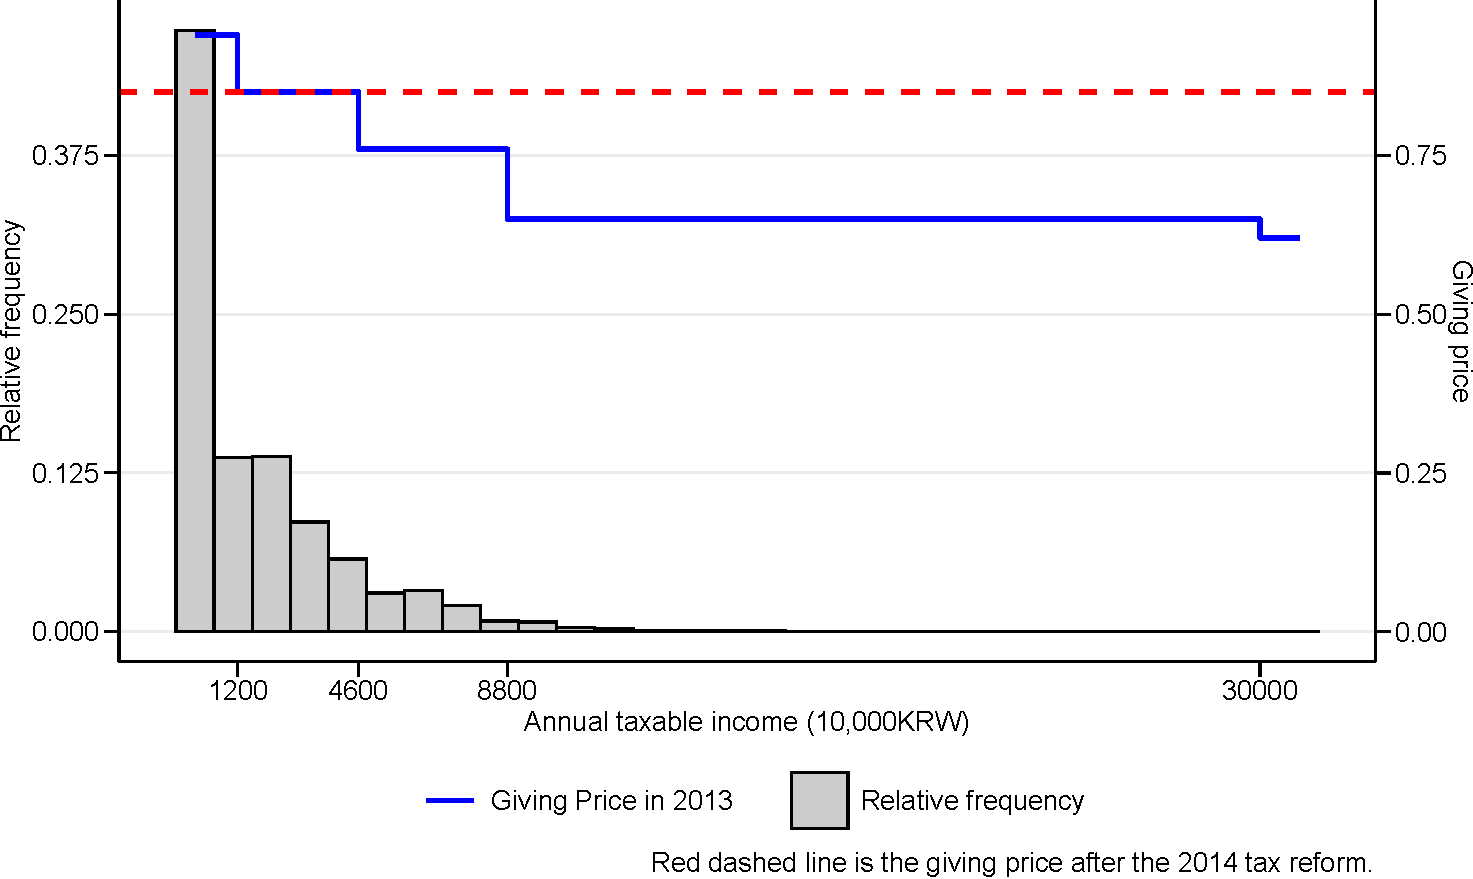
\includegraphics[width=0.85\linewidth]{C:/Users/vge00/Desktop/NASTAB/report/slide_files/figure-beamer/SummaryPriceChange-1} 

}

\caption{Income Distribution and Giving Price in 2013}\label{fig:SummaryPriceChange}
\end{figure}
\end{frame}

\begin{frame}{Fixed Effect Model}
\protect\hypertarget{fixed-effect-model}{}
The intensive-margin elasticity

\begin{equation}
    \ln g_{it} = \varepsilon^{int}_p R_{it} \ln p_{it} + \varepsilon^{int}_y \ln y_{it} 
    + X_{it}\beta +\mu_i +\iota_t +u_{it}. \label{eq:intensive}
\end{equation}

The extensive-margin elasticity

\begin{equation}
D_{it} =  \delta R_{it} \ln p_{it} +\gamma \ln y_{it} + X_{it}\beta +\mu_i  +\iota_t +v_{it}. \label{eq:extensive}
\end{equation}

\begin{itemize}
\tightlist
\item
  Since we use the linear probability model, the estimated coefficient \(\delta\) represents \(\hat{\delta} = \frac{\partial D_{it}}{\partial p_{it}} p_{it}\).
\item
  the implied extensive-margin price are calculated by \(\hat{\delta}/\bar{D}\) where \(\bar{D}\) is sample average of outcome variable \(D_{it}\).
\end{itemize}
\end{frame}

\begin{frame}{ITT approach and IV approach}
\protect\hypertarget{itt-approach-and-iv-approach}{}
\textbf{ITT approach = True price effect + Effect of self-selection of a tax relief}

\begin{itemize}
\tightlist
\item
  We assume that \(R_{it} = 1\) for all \(i\) and \(t\).
\end{itemize}

\textbf{IV approach = True price effect}

\begin{itemize}
\tightlist
\item
  First, using the emplyed dummy as IV, we estimate the following model:
\end{itemize}

\begin{align}
  R_{it}
  = \alpha_{1i} + \lambda \text{Employed}_{it} + X_{it} \beta_1
  + \mu_{i1} + \iota_{t1} + \eta_{it} \label{eq:stage1}
\end{align}

\begin{itemize}
\tightlist
\item
  There is a difference of declaration cost of tax relief since self-employed workers have to retain the certificate until they submit tax return although wage earners can submit the certificate at any time.\\
\item
  Second, we obtain the fitted value of \(R_{it}\) (\(\hat{R}_{it}\)) and replace \(R_{it}\) with \(\hat{R}_{it}\).
\end{itemize}
\end{frame}

\begin{frame}{Results: ITT Approach}
\protect\hypertarget{results-itt-approach}{}
\begin{table}
\centering\begingroup\fontsize{9}{11}\selectfont

\begin{tabular}{lccc}
\toprule
 & Overall & Intensive & Extensive\\
\midrule
$\hat{\varepsilon}_p^{int}$ & -1.241*** & -0.904*** & \\
 & (0.227) & (0.249) & \\
$\hat{\delta}$ &  &  & -0.267***\\
 &  &  & (0.051)\\
$\hat{\delta}/\bar{D}$ &  &  & -1.221***\\
 &  &  & (0.235)\\
Individual FE & Y & Y & Y\\
Time FE & Y & Y & Y\\
Age & Y & Y & Y\\
Year x Education & Y & Y & Y\\
Year x Gender & Y & Y & Y\\
Year x Resident Area & Y & Y & Y\\
N & 53267 & 11637 & 53267\\
Adjusted R-squared & 0.530 & 0.678 & 0.462\\
\bottomrule
\end{tabular}
\endgroup{}
\end{table}
\end{frame}

\begin{frame}{Results: IV Approach}
\protect\hypertarget{results-iv-approach}{}
\begin{table}
\centering\begingroup\fontsize{9}{11}\selectfont

\begin{tabular}{lccc}
\toprule
 & Overall & Intensive & Extensive\\
\midrule
$\hat{\varepsilon}_p^{int}$ & -1.603*** & -0.987*** & \\
 & (0.466) & (0.342) & \\
$\hat{\delta}$ &  &  & -0.319***\\
 &  &  & (0.110)\\
$\hat{\delta}/\bar{D}$ &  &  & -0.926***\\
 &  &  & (0.320)\\
Individual and time FE & Y & Y & Y\\
log(income) & Y & Y & Y\\
Age & Y & Y & Y\\
Year x Education & Y & Y & Y\\
Year x Gender & Y & Y & Y\\
Year x Resident Area & Y & Y & Y\\
Year x Dummy of industry & Y & Y & Y\\
N & 16946 & 5840 & 16946\\
Adjusted R-squared & 0.514 & 0.697 & 0.428\\
\bottomrule
\end{tabular}
\endgroup{}
\end{table}
\end{frame}

\begin{frame}{Conclusions}
\protect\hypertarget{conclusions}{}
Main message

\begin{itemize}
\tightlist
\item
  Both ITT approach and IV approach show that the giving price elasticity in Korea is around -1.
\item
  It implies that the effect from the declaration cost, which has been ignored, is not so large in South Korea.
\end{itemize}
\end{frame}

\begin{frame}{References}
\protect\hypertarget{references}{}
\hypertarget{refs}{}
\begin{CSLReferences}{1}{0}
\leavevmode\vadjust pre{\hypertarget{ref-Almunia2020}{}}%
Almunia, M., Guceri, I., Lockwood, B., Scharf, K., 2020. More giving or more givers? The effects of tax incentives on charitable donations in the UK. Journal of Public Economics 183. doi:\href{https://doi.org/10.1016/j.jpubeco.2019.104114}{10.1016/j.jpubeco.2019.104114}

\leavevmode\vadjust pre{\hypertarget{ref-Auten2002}{}}%
Auten, G.E., Sieg, H., Clotfelter, C.T., 2002. Charitable giving, income, and taxes: An analysis of panel data. American Economic Review 92, 371--382.

\leavevmode\vadjust pre{\hypertarget{ref-Bakija2011}{}}%
Bakija, J., Heim, B.T., 2011. How does charitable giving respond to incentives and income? New estimates from panel data. National Tax Journal 64, 615--650. doi:\href{https://doi.org/10.17310/ntj.2011.2S.08}{10.17310/ntj.2011.2S.08}

\leavevmode\vadjust pre{\hypertarget{ref-Fack2010}{}}%
Fack, G., Landais, C., 2010. Are tax incentives for charitable giving efficient? Evidence from france. American Economic Journal - Economic Policy 2, 117--141. doi:\href{https://doi.org/10.1257/pol.2.2.117}{10.1257/pol.2.2.117}

\leavevmode\vadjust pre{\hypertarget{ref-Randolph1995}{}}%
Randolph, W.C., 1995. Dynamic income, progressive taxes, and the timing of charitable contributions. Journal of Political Economy 103, 709--738. doi:\href{https://doi.org/10.1086/262000}{10.1086/262000}

\end{CSLReferences}
\end{frame}

\end{document}
